\documentclass[12pt, a4paper]{article}

% --- Packages ---
\usepackage[utf8]{inputenc}
\usepackage[margin=1in]{geometry}
\usepackage{graphicx}
\usepackage{hyperref}
\usepackage{tikz}
\usetikzlibrary{shapes.geometric, arrows, positioning, fit, calc}
\usepackage{listings}
\usepackage{xcolor}
\usepackage{titlesec}
\usepackage{enumitem}
\usepackage{tocloft}
\usepackage{float}

% --- Custom Colors & Styles ---
\definecolor{rosblue}{RGB}{34, 49, 79}
\definecolor{rospink}{RGB}{244, 114, 116}
\definecolor{codebg}{RGB}{245, 245, 245}

\lstdefinestyle{mystyle}{
    backgroundcolor=\color{codebg},   
    commentstyle=\color{green!60!black},
    keywordstyle=\color{blue},
    stringstyle=\color{rospink},
    basicstyle=\ttfamily\footnotesize,
    breaklines=true,                 
    captionpos=b,                    
    keepspaces=true,                 
    numbers=left,                    
    numbersep=5pt,                  
    showspaces=false,                
    showstringspaces=false,
    showtabs=false,                  
    tabsize=2
}
\lstset{style=mystyle}

% --- TikZ Styles ---
\tikzstyle{hw} = [rectangle, rounded corners, minimum width=3cm, minimum height=1cm,text centered, draw=black, fill=orange!30]
\tikzstyle{fw} = [rectangle, rounded corners, minimum width=3cm, minimum height=1cm,text centered, draw=black, fill=green!30]
\tikzstyle{sw} = [rectangle, rounded corners, minimum width=3cm, minimum height=1cm,text centered, draw=black, fill=rosblue!30, text=white]
\tikzstyle{arrow} = [thick,->,>=stealth]
\tikzstyle{line} = [thick,-]

% --- Title Page ---
\title{
    \vspace{-2cm}
    \rule{\textwidth}{1pt}\\[0.5cm]
    \Huge \textbf{UGVC-10: Comprehensive System Architecture \& Engineering Manual}\\
    \Large \textit{A Step-by-Step Guide to the Rover's Hardware, Firmware, and Software}\\
    \rule{\textwidth}{1pt}
}
\author{\textbf{Yusuf Borham} \\ Chief Technology Officer (CTO) \\ AUR Technical Team}
\date{May 2026}

\begin{document}

\maketitle
\thispagestyle{empty}

\begin{abstract}
\noindent This document serves as the master engineering manual for the UGVC-10 Unmanned Ground Vehicle. It explains the entire system from the flow of electricity on the PCBs, to the embedded C code on the STM32, up to the high-level Artificial Intelligence and ROS 2 Navigation stack on the Raspberry Pi. Sub-team members must read their respective sections to understand how their work integrates into the larger system.
\end{abstract}

\newpage
\tableofcontents
\newpage

% ==========================================
% SECTION 1: SYSTEM OVERVIEW
% ==========================================
\section{Master System Overview}
Building a complex robotic system requires separating the "Brain" from the "Muscles." If the Brain (Raspberry Pi) tries to do muscle work (sending high-speed PWM to motors), it will fail. If the Muscles (STM32) try to do brain work (Computer Vision), they will crash.

\subsection{The Three Layers of the Rover}
\begin{enumerate}
    \item \textbf{Layer 0 (Hardware):} The skeleton, cardiovascular system, and muscles. Handles raw power, electrical isolation, and physical movement.
    \item \textbf{Layer 1 (Firmware/STM32):} The spinal cord. Handles real-time reflexes, reads raw sensors instantly, and keeps the motors spinning at exact speeds.
    \item \textbf{Layer 2 (Software/ROS 2):} The brain. Looks at cameras, builds 3D maps, makes decisions, and tells the spinal cord where to go.
\end{enumerate}

\begin{figure}[H]
\centering
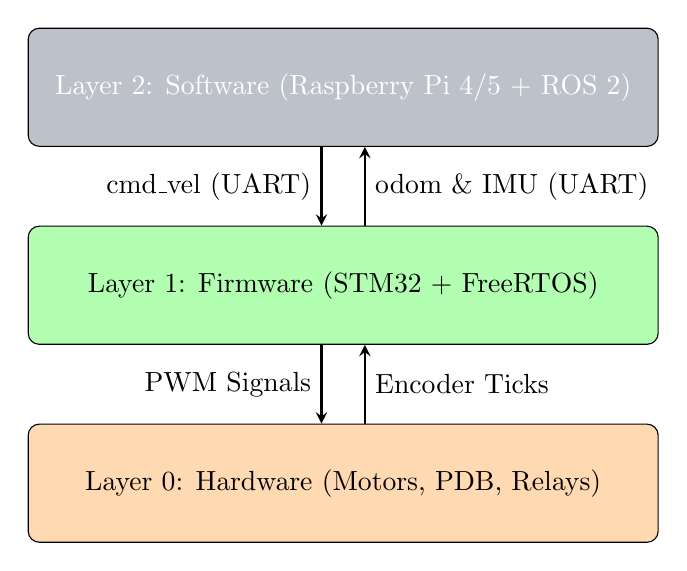
\begin{tikzpicture}
    % Nodes
    \node (pi) [sw, minimum width=8cm, minimum height=1.5cm] {Layer 2: Software (Raspberry Pi 4/5 + ROS 2)};
    \node (stm) [fw, below=1cm of pi, minimum width=8cm, minimum height=1.5cm] {Layer 1: Firmware (STM32 + FreeRTOS)};
    \node (hw) [hw, below=1cm of stm, minimum width=8cm, minimum height=1.5cm] {Layer 0: Hardware (Motors, PDB, Relays)};
    
    % Arrows
    \draw [arrow] (pi.250) -- node[anchor=east] {cmd\_vel (UART)} (stm.110);
    \draw [arrow] (stm.70) -- node[anchor=west] {odom \& IMU (UART)} (pi.290);
    
    \draw [arrow] (stm.250) -- node[anchor=east] {PWM Signals} (hw.110);
    \draw [arrow] (hw.70) -- node[anchor=west] {Encoder Ticks} (stm.290);
\end{tikzpicture}
\caption{High-Level Architecture and Data Flow}
\end{figure}

\newpage

% ==========================================
% SECTION 2: HARDWARE (LAYER 0)
% ==========================================
\section{Hardware Architecture (Layer 0)}
The Hardware team is responsible for ensuring the system does not catch fire, does not suffer from sensor noise, and complies with UGVC safety rules.

\subsection{Power Distribution Board (PDB)}
The main battery is 24V. We must drop this voltage safely.
\begin{itemize}
    \item \textbf{24V Rail:} Goes directly to the custom Motor Drivers. This is a high-noise environment.
    \item \textbf{5V Rail (Buck Converter):} Powers the Raspberry Pi and the Lidar. Must provide at least 5 Amps to prevent the Pi from rebooting under heavy CPU load.
    \item \textbf{3.3V Rail (Buck Converter):} Powers the STM32, GPS module, and IMU (BNO055). This must be ultra-clean power to prevent sensor drift.
\end{itemize}

\subsection{The Safety E-Stop Circuit (Crucial)}
The UGVC rules require two E-Stops (Mechanical and Wireless) that are \textbf{hardware-based}.
\begin{itemize}
    \item \textbf{How it works:} The 24V battery ground wire runs through a heavy-duty relay/contactor before reaching the motor drivers.
    \item \textbf{Mechanical Switch:} A big red button on the back of the rover. Hitting it opens the relay.
    \item \textbf{Wireless Switch:} A 2.4GHz LoRa/NRF receiver sits on the rover. If the judge presses the remote, the receiver pulls a pin LOW, which opens the relay.
    \item \textit{Note:} The Raspberry Pi and STM32 remain powered on when the E-stop is hit. Only the motors lose power. This prevents us from having to reboot the whole computer during a safety pause.
\end{itemize}

\subsection{Logic Level Shifting}
The STM32 operates at 3.3V. The Motor Drivers likely require 5V PWM signals. If you connect them directly, the signals will fail or fry the board. Hardware must place \textbf{Bi-Directional Logic Level Converters} between the STM32 and the Motor Drivers.

\subsection{Control Board (STM32)}
The Control Board is based on the STM32 microcontroller, which serves as the central processing unit for the firmware layer.

\begin{itemize}
    \item \textbf{Microcontroller:} STM32F4 series (e.g., STM32F407) for its balance of performance and power efficiency.
    \item \textbf{Communication:} UART for communication with the Raspberry Pi, I2C for sensors, and PWM outputs for motor control.
    \item \textbf{Sensors:} Encoders for wheel speed, IMU (BNO055) for orientation, and GPS module for global positioning.
\end{itemize}

\subsection{Home Made Motor Driver Boards or BTS }
\begin{itemize}
    \item \textbf{Motor Drivers:} We use either custom-built H-Bridge motor drivers or off-the-shelf BTS7960 modules, which can handle the high current required by the motors.
    \item \textbf{Features:} These drivers support PWM control for speed regulation and direction control, as well as built-in protection against overcurrent and overheating.
    \item Also we might need to measure current for better control and safety, so we can add current sensors (like ACS712) to the motor driver circuit.
\end{itemize}

\newpage

% ==========================================
% SECTION 3: FIRMWARE (LAYER 1)
% ==========================================
\section{Firmware Architecture (STM32)}
The STM32 runs on \textbf{FreeRTOS} (Real-Time Operating System). Instead of one giant loop, FreeRTOS splits the code into "Tasks" that run concurrently based on priority.

\subsection{FreeRTOS Task Map}
\begin{figure}[H]
\centering
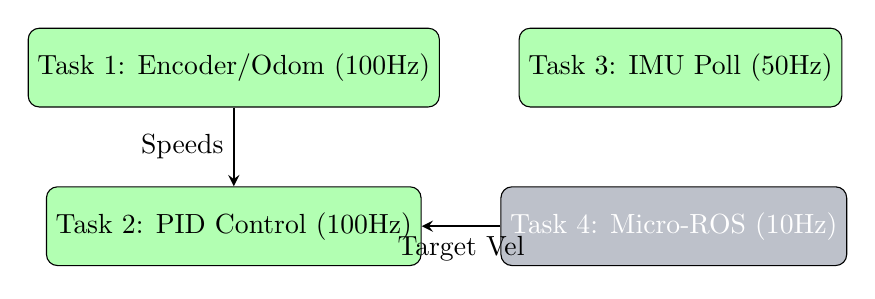
\begin{tikzpicture}
    \node (enc) [fw] {Task 1: Encoder/Odom (100Hz)};
    \node (pid) [fw, below=1cm of enc] {Task 2: PID Control (100Hz)};
    \node (imu) [fw, right=1cm of enc] {Task 3: IMU Poll (50Hz)};
    \node (ros) [sw, right=1cm of pid] {Task 4: Micro-ROS (10Hz)};
    
    \draw [arrow] (enc) -- node[anchor=east] {Speeds} (pid);
    \draw [arrow] (ros) -- node[anchor=north] {Target Vel} (pid);
\end{tikzpicture}
\caption{STM32 RTOS Task Priorities}
\end{figure}

\subsection{Embedded APIs and Drivers}
Here is exactly how the STM32 interacts with the hardware components:

\subsubsection{Encoder Driver (Hardware Timers)}
We do not use software interrupts for encoders; it is too slow. We use STM32 Hardware Timers in Encoder Mode.
\begin{itemize}
    \item \textbf{API:} \texttt{HAL\_TIM\_Encoder\_Start(\&htim1, TIM\_CHANNEL\_ALL);}
    \item \textbf{Logic:} Read the timer counter (\texttt{\_\_HAL\_TIM\_GET\_COUNTER}) every 10ms. Subtract the old value from the new value. Convert those raw ticks into RPM, and then into linear wheel velocity (m/s) using the wheel radius.
\end{itemize}

\subsubsection{Motor Control (PWM )}
The STM32 receives a target $V_x$ (forward speed) and $\omega_z$ (turning speed) from ROS 2.
\begin{itemize}
    \item \textbf{Kinematics:} We calculate what each wheel should do.
    $$ V_{left} = V_x - (\omega_z \times \frac{Track\_Width}{2}) $$
    $$ V_{right} = V_x + (\omega_z \times \frac{Track\_Width}{2}) $$
    \item \textbf{API:} \texttt{\_\_HAL\_TIM\_SET\_COMPARE(\&htim3, TIM\_CHANNEL\_1, pwm\_value);}
\end{itemize}

\subsubsection{Kinematic equation for the rover}
The rover is a differential drive robot. The kinematic equations are:
$$ V_x = \frac{V_{left} + V_{right}}{2} $$
$$ \omega_z = \frac{V_{right} - V_{left}}{Track\_Width} $$

These speeds are sent to the PI for the odom message and for the EKF.

\subsubsection{IMU Driver (BNO055 via I2C)}
The BNO055 does sensor fusion internally.
\begin{itemize}
    \item \textbf{API:} \texttt{HAL\_I2C\_Mem\_Read(\&hi2c1, BNO\_ADDR, REG, 1, buffer, size, timeout);}
    \item \textbf{Logic:} We read the Quaternion registers to get the absolute Heading (Yaw), and the Gyroscope registers to get rotational velocity ($\omega_z$).
\end{itemize}

\subsubsection{Laser Pointer \& Servo Drivers}
\begin{itemize}
    \item \textbf{Laser:} Just a standard GPIO pin. \texttt{HAL\_GPIO\_WritePin(PORT, PIN, GPIO\_PIN\_SET);} triggered when ROS 2 says "Face Found."
    \item \textbf{Servo:} Uses a Timer configured for PWM. Modifying the duty cycle changes the angle of the upward-facing camera.
\end{itemize}

\subsubsection{ GPS API}
\begin{itemize}
    \item \textbf{Module:} We use a u-blox NEO-M8N GPS with RTK capability.
    \item \textbf{Data:} The GPS outputs NMEA sentences over UART. We parse these to extract Latitude, Longitude, and Altitude.
\end{itemize}

\subsubsection{Communication Module For the PI}
\begin{itemize}
    \item \textbf{Module:} We use a STM32-based communication module to interface with the Raspberry Pi.
    \item \textbf{Data:} The module handles the wired communication between the STM32 and the Raspberry Pi.
\end{itemize}

\subsubsection{PID Control for wheel velocity}
\begin{itemize}
    \item \textbf{Logic:} The PID controller runs at 100Hz. It takes the target wheel velocities from ROS 2 and compares them to the actual velocities from the encoders. The error is processed through the PID algorithm to generate the appropriate PWM signals for the motors.
    \item It must be tuned carefully to ensure smooth acceleration and deceleration without overshooting or oscillations.
    \item \textbf{API:} The PID output is sent to the motor drivers using the STM32's PWM capabilities, ensuring precise control over the motor speeds.
    \item Must also include anti windup mechanisms to prevent the integral term from accumulating excessively when the motors are saturated.
    \item also must have a high pass filter on the derivative term to prevent noise from causing erratic motor behavior.
\end{itemize}

\subsubsection{Bluetooth Module for Remote Control}
\begin{itemize}
    \item \textbf{Module:} We use a Bluetooth module (e.g., HC-05) for remote control and diagnostics.
    \item \textbf{Data:} The module allows for wireless communication between the STM32 and a smartphone or laptop, enabling manual control and real-time monitoring of sensor data, or for taking the robot from one place to another without having to start the whole system up againn

\end{itemize}

\subsubsection{ Voltage and Current measurement code }

\begin{itemize}
    \item Probably we will use a voltage divider with a protection circuit with an ADC pin on the STM32 to measure the battery voltage. For current measurement, we can use a current sensor like the ACS712, which outputs an analog voltage proportional to the current flowing through it. The STM32 can read this voltage using its ADC to calculate the current draw of the motors and other components,or we can add a shunt resistor in series with the motor power line and measure the voltage drop across it to calculate current using Ohm's Law (I = V/R).
\end{itemize}

\newpage



% ==========================================
% SECTION 4: SOFTWARE (LAYER 2 - ROS 2)
% ==========================================
\section{Software Architecture (ROS 2 Humble/Jazzy)}
The Raspberry Pi handles all the complex AI, mapping, and decision-making.

\subsection{The ROS 2 Workspace (\texttt{ugvc\_ws})}
The workspace must be strictly organized into these packages:
\begin{itemize}
    \item \textbf{\texttt{ugvc\_description}:} Contains the URDF file. This is an XML file that tells ROS 2 exactly where every sensor is physically bolted on the robot (e.g., "The GPS is 20cm behind the center of the wheels").
    \item \textbf{\texttt{ugvc\_hardware}:} Runs the \texttt{micro\_ros\_agent} to talk to the STM32.
    \item \textbf{\texttt{ugvc\_vision}:} Contains the Python OpenCV and YOLOv8 scripts.
    \item \textbf{\texttt{ugvc\_navigation}:} Contains the Kalman Filters, Costmaps, and Path Planners.
\end{itemize}

\subsection{ROS 2 Node \& Topic Dictionary}
This is the lifeblood of the system. Every team member must know what data is flowing where.

\begin{figure}[H]
\centering
{
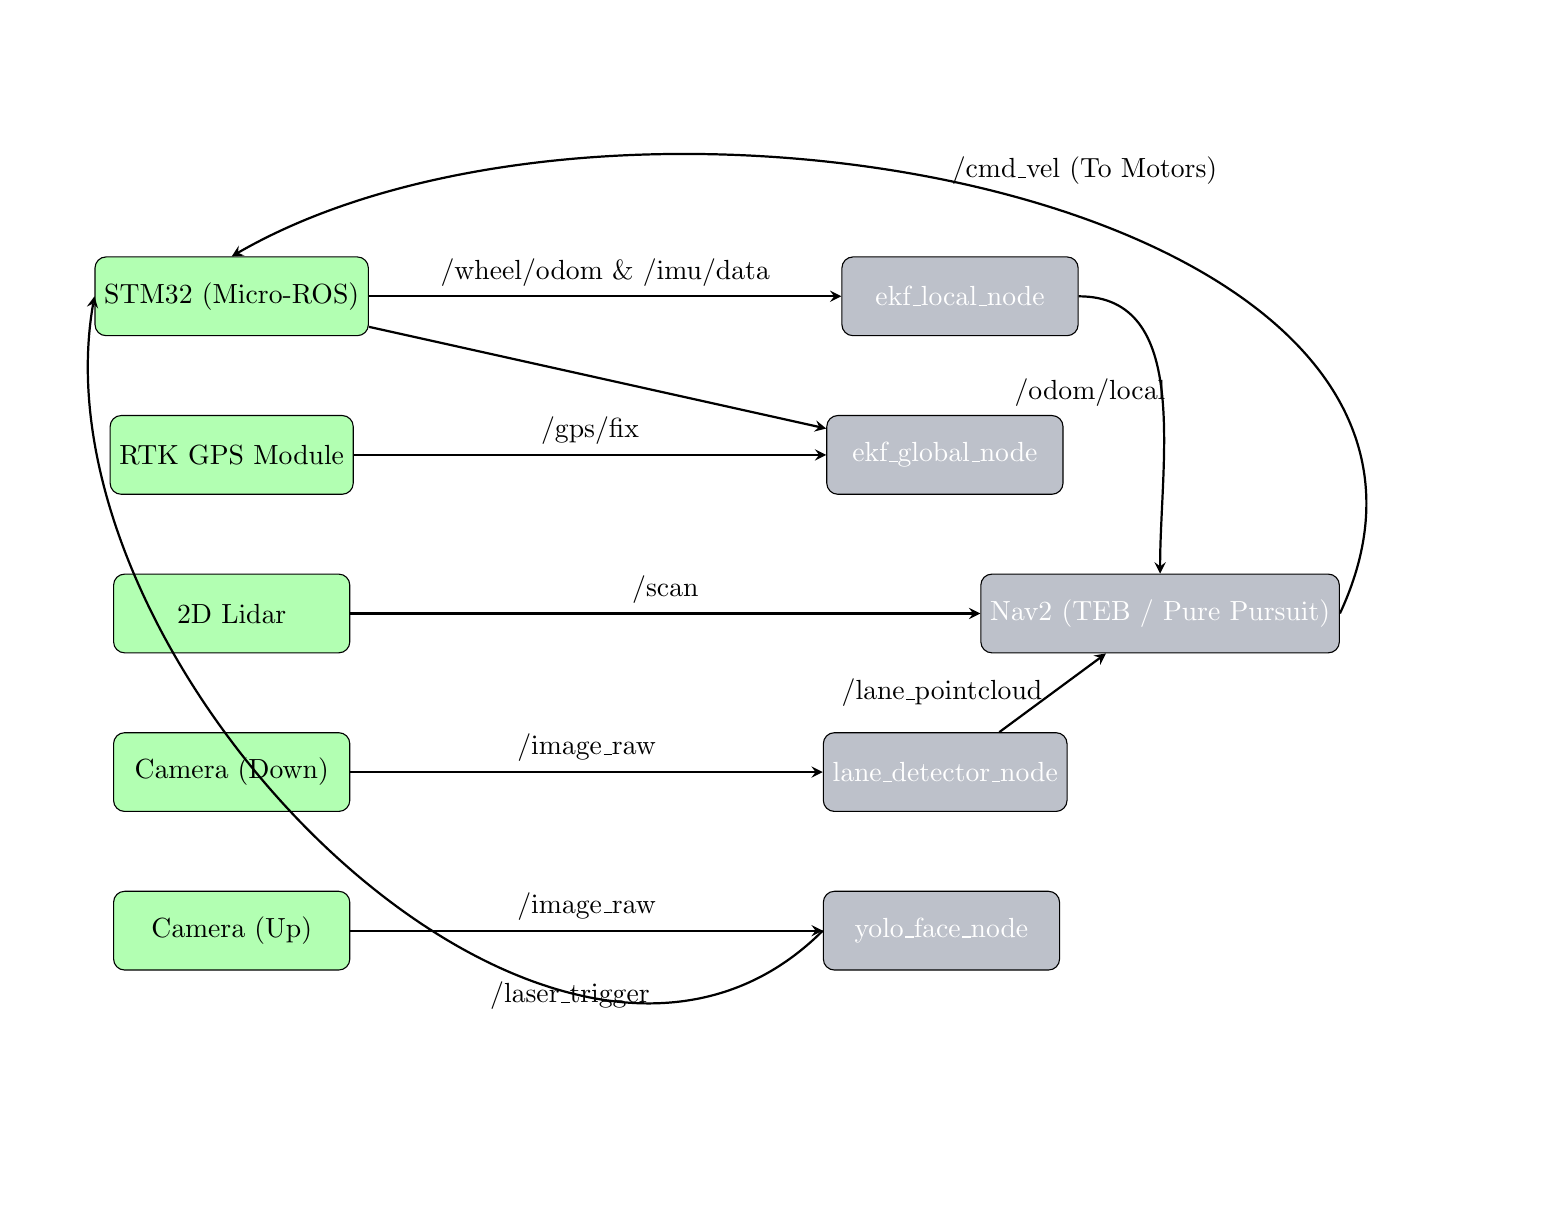
\begin{tikzpicture}[scale=1, transform shape]
    % Hardware/Sensors (Inputs)
    \node (stm) [fw] {STM32 (Micro-ROS)};
    \node (gps) [fw, below=1cm of stm] {RTK GPS Module};
    \node (lidar) [fw, below=1cm of gps] {2D Lidar};
    \node (camd) [fw, below=1cm of lidar] {Camera (Down)};
    \node (camu) [fw, below=1cm of camd] {Camera (Up)};

    % ROS Nodes (Processing)
    \node (ekfl) [sw, right=6cm of stm] {ekf\_local\_node};
    \node (ekfg) [sw, right=6cm of gps] {ekf\_global\_node};
    \node (nav) [sw, right=8cm of lidar] {Nav2 (TEB / Pure Pursuit)};
    \node (lane) [sw, right=6cm of camd] {lane\_detector\_node};
    \node (yolo) [sw, right=6cm of camu] {yolo\_face\_node};

    % Arrows & Topics
    \draw [arrow] (stm) -- node[anchor=south] {/wheel/odom \& /imu/data} (ekfl);
    \draw [arrow] (stm) -- (ekfg);
    \draw [arrow] (gps) -- node[anchor=south] {/gps/fix} (ekfg);
    \draw [arrow] (lidar) -- node[anchor=south] {/scan} (nav);
    \draw [arrow] (camd) -- node[anchor=south] {/image\_raw} (lane);
    \draw [arrow] (camu) -- node[anchor=south] {/image\_raw} (yolo);

    \draw [arrow] (lane) -- node[anchor=east] {/lane\_pointcloud} (nav);
    \draw [arrow] (ekfl.east) to[out=0,in=90] node[anchor=west , xshift=-2cm] {/odom/local} (nav.north);
    
    \draw [arrow] (nav.east) to[out=65,in=30] node[anchor=south, xshift=1cm] {/cmd\_vel (To Motors)} (stm.north);
    \draw [arrow] (yolo.west) to[out=-135,in=-100] node[anchor=north, xshift=3cm , yshift=-1.5cm] {/laser\_trigger} (stm.west);

\end{tikzpicture}
}
\caption{Complete ROS 2 Node and Topic Architecture}
\end{figure}

\subsection{GUI }
We have a custom GUI built with \textbf{rqt} that shows:
\begin{itemize}
    \item Real-time camera feeds with lane detection and face bounding boxes.
    \item A live-updating map with the rover's position, Lidar obstacles, and planned path.
    \item Diagnostic data like wheel speeds, GPS coordinates, and IMU readings.
\end{itemize}

\subsection{Network Architecture}
The Raspberry Pi runs a ROS 2 \textbf{DDS} (Data Distribution Service) network. All nodes communicate over this network using topics. The micro-ROS agent or the pyserial on the STM32 bridges the hardware data into this network.

A long Range router to allow the station to be connected to the rover from a disatnce for the camera feed and the manual control if needed.

\newpage

% ==========================================
% SECTION 5: AUTONOMY ALGORITHMS (HOW IT THINKS)
% ==========================================
\section{The Autonomy Engine: How We Win}

\subsection{Step 1: Localization (Where am I?)}
We use the \textbf{Extended Kalman Filter (EKF)} from the \texttt{robot\_localization} package.
\begin{itemize}
    \item \textbf{Local EKF:} Fuses the Encoders + IMU. It provides a super smooth 50Hz location update so the rover doesn't jerk around obstacles.
    \item \textbf{Global EKF:} Fuses Encoders + IMU + RTK GPS. This locks the rover to the exact Earth coordinates to hit the 1.5m waypoint target.
\end{itemize}

\subsection{Step 2: Perception (What is around me?)}
The UGVC course has physical objects, flat painted white lines, and flat white potholes.
\begin{itemize}
    \item \textbf{The Lidar:} Maps the 3D physical obstacles into the ROS 2 \textbf{Costmap}.
    \item \textbf{The Downward Camera:} Runs an OpenCV Python script. It masks the image for pure white. It uses \texttt{cv2.warpPerspective} to flatten the image (Bird's Eye View). It then publishes the white pixels as a fake 3D Pointcloud.
    \item \textbf{The Result:} The ROS 2 Costmap merges the Lidar and the Camera data. To the path planner, a flat white painted line looks exactly like a 10-foot brick wall. It will not cross it.
\end{itemize}

\subsection{Step 3: Planning (How do I move?)}
\begin{itemize}
    \item \textbf{Global Planner (A* or Dijkstra):} Draws the shortest line from where we are to the GPS waypoint.
    \item \textbf{Local Planner (TEB Local Planner):} Looks at the Costmap and the Global Path. It bends the path around the obstacles and white lines dynamically. It guarantees we stay between 2 km/hr and 10 km/hr and don't accelerate too fast.
\end{itemize}

\subsection{Step 4: The State Machine (Behavior Trees)}
We do not use messy "if/else" statements in Python. We use Nav2 \textbf{Behavior Trees (XML)}.
\begin{enumerate}
    \item \textbf{Bounded Track Mode:} Use Lidar + Camera + TEB Planner to dodge obstacles.
    \item \textbf{Unbounded Waypoint Mode:} Turn off Cameras. Turn off TEB. Use \textbf{Pure Pursuit} to drive full speed directly to the GPS coordinates (because this area is obstacle-free).
    \item \textbf{Waypoint 2 (Image Detection):} 
    \begin{itemize}
        \item Halt \texttt{cmd\_vel}.
        \item Trigger STM32 to sweep the servo.
        \item \texttt{yolo\_face\_node} looks for the target dummy.
        \item When found, publish \texttt{True} to \texttt{/laser\_trigger}.
        \item Wait 3 seconds, resume driving to Waypoint 3.
    \end{itemize}
\end{enumerate}

\end{document}